% !TeX Options = -shell-escape

\documentclass[10pt]{beamer}

\usetheme[progressbar=frametitle, block=fill]{metropolis}
\usepackage{xcolor}
\usepackage{multirow}
\usepackage{pgfpages}
\usepackage{pifont}
\usepackage[utf8]{inputenc}
\usepackage[T1]{fontenc}
\usepackage[english]{babel}
\newcommand{\cmark}{\ding{51}}
\newcommand{\xmark}{\ding{55}}
\setbeamertemplate{note page}{\insertnote}
%\setbeameroption{show notes on second screen=left}
\setbeameroption{hide notes}
\definecolor{amethyst}{rgb}{0.5, 0.4, 1.0}
\definecolor{amethystgrey}{rgb}{0.85, 0.85, 1.0}
\definecolor{amethystdark}{rgb}{0.4, 0.3, 0.9}
\definecolor{orangedark}{rgb}{0.0, 0.9, 0}
%\definecolor{titlebg}{HTML}{4e8074}
%\definecolor{titlebg}{HTML}{3e7985}
\definecolor{titlebg}{HTML}{fbf8ff}
\definecolor{font}{HTML}{23373b}
%\setbeamercolor{title}{fg=amethyst, bg=amethyst}
\setbeamercolor{frametitle}{fg= font, bg=titlebg}
%\setbeamercolor{section title}{black}
%\setbeamercolor{structure}{fg=amethyst, bg=amethyst}
\setbeamercolor{progress bar}{ fg = amethyst, bg= amethystgrey }
%\setbeamercolor{itemize item}{fg=amethyst,bg=white}
\setbeamercolor{alerted text}{fg=amethystdark}
%\setbeamercolor{title separator}{ ... }
%\setbeamercolor{progress bar in head/foot}{ ... }
%\setbeamercolor{progress bar in section page}{ ... }

\newcommand{\code}[1]{\texttt{#1}}

\usepackage{booktabs}
\usepackage[scale=2]{ccicons}

\usepackage{minted}

\usepackage{pgfplots}

\usepackage{xspace}

\title{Coroutines}
\subtitle{All you need to know about the coroutines}
\date{}
\author{Dawid Pilarski}
\institute{dawid.pilarski@tomtom.com \\ blog.panicsoftware.com}


\setminted[c++]
{
framesep=2mm,
baselinestretch=1.2,
fontsize=\footnotesize,
autogobble=true
}

\begin{document}

\maketitle

\begin{frame}{Agenda}
\tableofcontents
\end{frame}

\section{Coroutine theory - what are the coroutines?}

\begin{frame}{What are the coroutines?}
\alert{Coroutines} are \alert{generalization} of the function, that can be:

\begin{itemize}[<+- |alert@+>]
\item created
\item called
\item returned from
\item suspended
\item resumed
\item destroyed
\end{itemize}

\end{frame}

\begin{frame}{Coroutine flowchart}

\begin{columns}
\begin{column}{0.48\linewidth}
  \centering
  Function's flow:
  \vskip 2em
  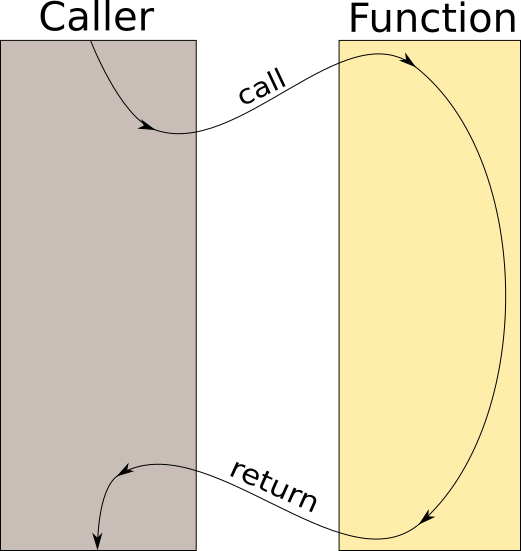
\includegraphics[width=0.8\linewidth]{graphics/function-call.png}
\end{column}

\begin{column}{0.48\linewidth}
  \centering
  Coroutine flow:
  \vskip 2em
  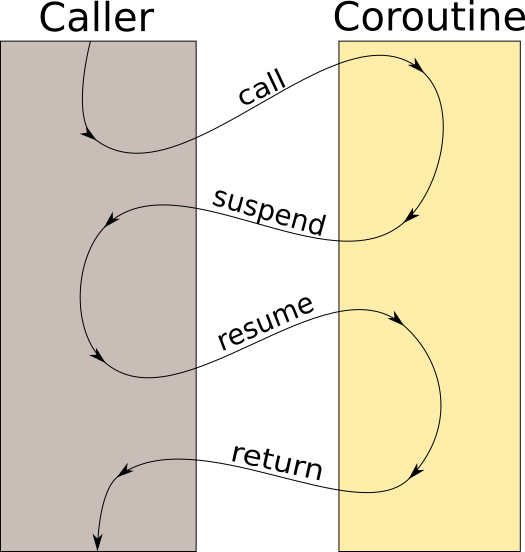
\includegraphics[width=0.8\linewidth]{graphics/coroutine-workflow.png}
\end{column}

\end{columns}

\end{frame}

\begin{frame}{Possible coroutines implementations}

\begin{columns}
\begin{column}{0.48\linewidth}
  Language based
\end{column}

\begin{column}{0.48\linewidth}
  Library based
\end{column}
\end{columns}

\end{frame}

\begin{frame}{Closer look into Boost.Fiber}
  \begin{itemize}[<+- |alert@+>]
  \item Need to allocate the stack for the Fiber/Coroutine
  \item Can be suspended from the top level functions and below
  \item Allocation of the memory in advance
  \item Hard to optimize by compilers
  \end{itemize}
\end{frame}

\begin{frame}{Closer look into built-in coroutines}
  \begin{itemize}[<+- |alert@+>]
  \item Need to allocate the stack for the Coroutine
  \item Can be suspended only from the top level functions
  \item Easy to optimize by compilers
  \item "Easy" to optimize by the compilers
  \end{itemize}
\end{frame}

\begin{frame}[fragile]{Coroutine declarations}
  \centering Same as functions

  \vfill
  \begin{center}
  \begin{minipage}{0.7\linewidth}
  \inputminted{c++}{code-examples/intro/declaration.hpp}
  \end{minipage}
  \end{center}
  \vfill

  Whether the function is a coroutine depends on it's definition.

\end{frame}

\begin{frame}{3 new keywords}
  \begin{description}
    \item [\code{co\_return}] \hfill \\ Returning (or not) value and finishing the coroutine
    \item [\code{co\_yield}] \hfill \\ Returning intermediate value from the coroutine
    \item [\code{co\_await}] \hfill \\ Awaiting completion of the "task"
  \end{description}
\end{frame}

\section{Practical part I - using cppcoro}

\begin{frame}{generators}
  \inputminted[firstline=3]{c++}{code-examples/cppcoro/generator.cpp}
\end{frame}

\begin{frame}{generators - excercise}
  % https://edublognss.wordpress.com/2013/04/16/famous-mathematical-sequences-and-series/
  \centering Implement any generator:

  \begin{itemize}
    \item square number series \hskip 2em 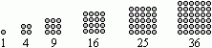
\includegraphics[width=0.3\linewidth]{graphics/square-series.png}
    \item triangular number series \hskip 2em 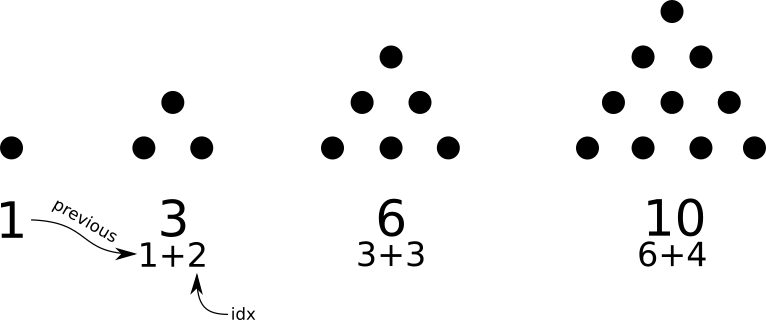
\includegraphics[width=0.3\linewidth]{graphics/triangular-series.png}
  \end{itemize}
\end{frame}

\begin{frame}{tasks and events}
  \inputminted[firstline=8]{c++}{code-examples/cppcoro/events.cpp}
\end{frame}

\begin{frame}{tasks and events excercise}
  What should be here?
\end{frame}

\begin{frame}{other (for now only msvc)}
  \begin{itemize}
    \item mutexes
    \item file I/O operations
    \item networking operations
  \end{itemize}
\end{frame}

\begin{frame}{other (for now only msvc)}
  \inputminted[firstline=4]{c++}{code-examples/cppcoro/io.cpp}
\end{frame}

\section{Theory - implementing own coroutines types}

\begin{frame}{promise\_type}
  \begin{itemize}[<+- |alert@+>]
    \item promise\_type is strongly connected with coroutine's returned type
    \begin{itemize}[<+- |alert@+>]
      \item it can be a member of the returned type \code{returned\_type::promise\_type}
      \item it can be defined as \code{std::coroutine\_traits<returned\_type>::promise\_type}
    \end{itemize}
    \item promise\_type is responsible for coroutine's behavior:
    \begin{itemize}
      \item on coroutine's start
      \item on throwing unhandled exception
      \item on coroutine's end
      \item on returning the value
      \item on yielding the value
      \item partially on waiting for the task's completion
    \end{itemize}
  
  \end{itemize}
\end{frame}

\begin{frame}{coroutine body}
\centerline{Each time we write coroutine, compiler modifies it's body into following form:}
\inputminted[firstline=1]{c++}{code-examples/theory-custom-coroutine/coroutine-body.cpp}
\end{frame}

\begin{frame}{promise\_type extensions}
\centerline{We can extend the coroutine body with:}
\begin{itemize}
  \item mandatory support for returning void or returning value
  \item custom memory allocation algorithm (custom \code{operator new})
  \item optional support for yielding intermediate values
\end{itemize}
\end{frame}

\begin{frame}[fragile]{co\_return}
\centerline{\alert{\code{co\_return}} is a new keyword}

\begin{columns}[T]
  \begin{column}{0.48\linewidth}
  \vskip 2em
  \centerline{Usage: }
  \vskip 2em
  \begin{onlyenv}<1>

  without expression:
  \begin{minted}{c++}
  co_return 
  \end{minted}

  with void expression:
  \begin{minted}{c++}
  co_return <void expression>
  \end{minted}

  \end{onlyenv}

  \begin{onlyenv}<2>
  with non-void expression:
  \begin{minted}{c++}
  co_return <expression>
  \end{minted}
  \end{onlyenv}

  \end{column}

  \begin{column}{0.48\linewidth}
  \vskip 2em
  \centerline{Translated to: }
  \vskip 2em
  \begin{onlyenv}<1>
   \begin{minted}{c++}
   <expression>;
   promise.return_void();
   goto final_suspend;
   \end{minted}
   \end{onlyenv}
   \begin{onlyenv}<2>
   \begin{minted}{c++}
   promise.return_value(<expression>);
   goto final_suspend;
   \end{minted}
   \end{onlyenv}

  \end{column}
\end{columns}
\end{frame}

\begin{frame}[fragile]{co\_yield}
\centerline{\alert{\code{co\_yield}} is a new keyword}

\begin{columns}
\begin{column}{0.48\linewidth}
\vskip 2em
Usage:
\vskip 2em

\begin{minted}{c++}
co_yield <non-void expression>
\end{minted}

\end{column}

\begin{column}{0.48\linewidth}
\vskip 2em
Translated to:
\vskip 2em

\begin{minted}{c++}
co_await promise.
         yield_value(<expression>)
\end{minted}

\end{column}
\end{columns}
\end{frame}

\begin{frame}{co\_await shortly}
\begin{description}
  \item[\code{co\_await std::experimental::suspend\_always\{\}}] - \hfill \\ suspends the coroutine
  \item[\code{co\_await std::experimental::suspend\_never\{\}}] - \hfill \\ does nothing
\end{description}

\end{frame}

\begin{frame}{co\_await}
\centerline{\alert{co\_await} is a new keyword}

\begin{itemize}
  \item represents awaiting for operations' completion
  \item it's argument is (usually) called awaitable
  \item it's result is usually called awaiter
\end{itemize}
\end{frame}

\begin{frame}{co\_await translation}
\centerline{If compiler meets the co\_await it gets translated into following code:}

\inputminted{c++}{code-examples/theory-custom-coroutine/co-await-transformation.cpp}
\end{frame}

\begin{frame}[fragile]{Await suspend}
% nothing yet said about the coroutine_handle
await suspend is of the following form:

\begin{minted}{c++}
promise.await_suspend(this_coroutine_handle);
\end{minted}

\code{await\_suspend} might return following types:
\vskip 1em
\hrule

\begin{columns}
\begin{column}{0.35\linewidth}
\begin{itemize}[<+- |alert@+>]
\item \code{void}
\item \code{bool}
\item \code{coroutine\_handle}
\end{itemize}
\end{column}

\begin{column}{0.66\linewidth}
\begin{onlyenv}<1>
\inputminted[firstline=1, lastline=9, linenos=false]{c++}{code-examples/theory-custom-coroutine/co-await-transformation-suspend.cpp}
\end{onlyenv}
\begin{onlyenv}<2>
\inputminted[firstline=10, lastline=22, linenos=false]{c++}{code-examples/theory-custom-coroutine/co-await-transformation-suspend.cpp}
\end{onlyenv}
\begin{onlyenv}<3>
\inputminted[firstline=23, linenos=false]{c++}{code-examples/theory-custom-coroutine/co-await-transformation-suspend.cpp}
\end{onlyenv}
\end{column}
\end{columns}

\end{frame}

\begin{frame}[fragile]{Awaitable and Awaiter}
\alert{Awaitable} is an object, which is an operand of the co\_await operator

\alert{co\_await <expression>} expression will be processed in following manner

\vskip 2em

\begin{columns}
\begin{column}{0.4\linewidth}
\begin{itemize}[<+- |alert@+>]
  \item await\_transform
  \item acquiring awaiter
  \begin{itemize}[<+- |alert@+>]
  \item co\_await operator
  \item global co\_await operator
  \item awaitable to awaiter
  \end{itemize}
\end{itemize}
\end{column}

\begin{column}{0.56\linewidth}
\footnotesize
\begin{onlyenv}<1>
  is performed only if promise has await\_transform function declared
  \vskip 2em

  \begin{minted}{c++}
  co_await promise.await_transform(<expr>);
  \end{minted}
\end{onlyenv}

\begin{onlyenv}<3>
  is performed only if awaitable has co\_await operator

  \begin{minted}{c++}
  auto&& awaiter = 
         <awaitable>.operator co_await();
  \end{minted}
\end{onlyenv}

\begin{onlyenv}<4>
  is performed only if awaitable there is matching global co\_await operator

  \begin{minted}{c++}
  auto&& awaiter = 
         operator co_await(<awaitable>);
  \end{minted}
\end{onlyenv}

\begin{onlyenv}<5>
  \begin{minted}{c++}
  auto&& awaiter = <awaitable>;
  \end{minted}
\end{onlyenv}

\end{column}
\end{columns}
\end{frame}

\section{Practical part II - implementing own coroutines types}

\begin{frame}{lazy}

\end{frame}

\begin{frame}{generator}

\end{frame}

\begin{frame}{task}

\end{frame}

\begin{frame}{event}

\end{frame}

\end{document}